\documentclass[11pt,a4paper]{article}

\usepackage[T1]{fontenc}
\usepackage[utf8]{inputenc}
\usepackage{lmodern}
\usepackage{microtype}
\usepackage{amsmath,amssymb,amsthm,mathtools,bm}
\usepackage{booktabs,array,tabularx,longtable,multirow}
\usepackage{graphicx,float,caption}
\usepackage{xcolor}
\usepackage[margin=23mm]{geometry}
\usepackage{enumitem}
\usepackage{fancyhdr}
\usepackage{hyperref}
\usepackage{pdflscape}
\usepackage{enumitem}

\definecolor{finblue}{HTML}{1F5A99}
\definecolor{finorange}{HTML}{C45A00}
\definecolor{fingreen}{HTML}{19733A}
\definecolor{finred}{HTML}{A61B1B}
\definecolor{finpurple}{HTML}{6B3FA0}
\definecolor{finsoft}{HTML}{F2F5F8}
\definecolor{fingray}{HTML}{4E5964}

\hypersetup{
  colorlinks=true,
  linkcolor=finblue,
  citecolor=fingreen,
  urlcolor=finblue,
  pdftitle={FIN Theory Compendium: From Fractal Information to the Current Mathematical Frontier},
  pdfauthor={Krzysztof Żuchowski},
  pdfsubject={A claim-graded reconstruction of the Fractal Information Theory project},
  pdfkeywords={FIN, fractal information, nadsoliton, spectral graph theory, dual dynamics, Green operator, Schur compression, information, operational physics}
}

\pagestyle{fancy}
\fancyhf{}
\fancyhead[L]{\small FIN Theory Compendium}
\fancyhead[R]{\small Release 10.48}
\fancyfoot[C]{\thepage}
\setlength{\headheight}{14pt}

\newtheorem{theorem}{Theorem}[section]
\newtheorem{proposition}[theorem]{Proposition}
\newtheorem{corollary}[theorem]{Corollary}
\theoremstyle{definition}
\newtheorem{definition}[theorem]{Definition}
\theoremstyle{remark}
\newtheorem{remark}[theorem]{Remark}

\newcommand{\C}{\mathbb C}
\newcommand{\R}{\mathbb R}
\newcommand{\Z}{\mathbb Z}
\newcommand{\one}{\bm 1}
\newcommand{\Tr}{\operatorname{Tr}}
\newcommand{\diag}{\operatorname{diag}}
\newcommand{\status}[2]{\textcolor{#1}{\textbf{[#2]}}}
\newcommand{\proven}{\status{fingreen}{PROVEN}}
\newcommand{\strong}{\status{finblue}{STRONG EVIDENCE}}
\newcommand{\moderate}{\status{finorange}{MODERATE EVIDENCE}}
\newcommand{\speculative}{\status{finpurple}{SPECULATIVE}}
\newcommand{\refuted}{\status{finred}{REFUTED}}
\newcommand{\conditional}{\status{fingray}{CONDITIONAL}}

\newcommand{\claimbox}[1]{%
  \begin{center}\fcolorbox{finblue}{finsoft}{\parbox{0.91\textwidth}{#1}}\end{center}}

\setlist[itemize]{leftmargin=*,topsep=3pt,itemsep=2pt}
\setlist[enumerate]{leftmargin=*,topsep=3pt,itemsep=2pt}
\setlength{\emergencystretch}{2em}

\begin{document}
\hypersetup{pageanchor=false}

\begin{titlepage}
\centering
\vspace*{16mm}
{\Huge\bfseries FIN Theory Compendium\par}
\vspace{5mm}
{\Large From Fractal Information and the Nadsoliton Idea\par}
\vspace{2mm}
{\Large to the Current Mathematical and Operational Frontier\par}
\vspace{14mm}
{\Large Krzysztof Żuchowski\par}
\vspace{2mm}
{\normalsize Independent Researcher --- Fractal Information Theory Project\par}
\vspace{2mm}
{\normalsize ORCID: 0009-0002-0909-3613\par}
\vspace{10mm}
{\large FIN Release 10.48 --- Version 1.0.0\par}
{\large 9 August 2026\par}
\vfill
\begin{minipage}{0.90\textwidth}
\small
\textbf{Purpose.} This document is a self-contained, claim-graded account of the whole FIN research programme: its originating physical intuition, the genealogy of the legacy and strict kernels, the results that survived mathematical falsification, the operational experiment specification, and the current exact-algebra frontier. It is a compendium, not a new claim of physical confirmation.

\medskip
\textbf{Epistemic boundary.} The project has no admitted independent laboratory record and no external scientific audit of the present release. All accepted results reported here are analytic, finite-dimensional, formal, interval-certified, or reproducible numerical statements within their declared models. Ontological and physical interpretations are labelled separately.

\medskip
\textbf{Repository.} \url{https://github.com/hyconiek/Fractal-Nadsoliton-Theory}

\textbf{License.} CC BY 4.0.
\end{minipage}
\vfill
\end{titlepage}
\hypersetup{pageanchor=true}

\begin{abstract}
FIN began from a radical ontological proposal: reality has one foundation, self-similar fractal information, existing as a persistent self-coupled ``nadsoliton.'' The founding picture further proposed that positive feedback sustains the informational excitation, that adaptive self-interaction resembles a self-learning neural network, and that light, matter and observers are emergent internal patterns. This document preserves that programme while separating it from what has actually been established.

The strongest present mathematical core is a finite, dimensionless spectral-information framework. On the strict twelve-state carrier, positive radial weights define a connected weighted graph Laplacian $A=sI-W\succeq0$. The same spectral resolution generates the unitary group $U_t=e^{-itA}$, the reversible Markov semigroup $P_t=e^{-tA}$, Green resolvents, source actions, exact Schur reductions, multiscale information geometry and conditional operational tests. Exact Green--Schur elimination rigorously realizes one form of fractal information compression, but neither produces the strict kernel from the legacy kernel nor creates an absolute length, time, action, mass or energy scale. Shannon information supports exact dimensionless identities and data-processing statements; it does not determine thermodynamic energy without an independently supplied Hamiltonian and calibration.

The historical legacy kernel is best retained as an intermediate bridge object. The later strict kernel is an operationally frozen enriched profile. A subsequent audit reconstructed the corrected Legacy* class, but did not create a third co-equal final kernel or prove a legacy-to-strict completion. The $\Z_{12}$ carrier, phase coherence, signed representation resources, exact process-tester optimization and a laboratory transfer specification are substantive achievements. By contrast, the historical Planck-layer hierarchy, particle-mass formulas, Standard Model identifications, gravity scaling and ``maximum resonance instead of minimum energy'' remain hypotheses or have been downgraded.

The deepest interpretation surviving current falsification is therefore not a completed physical theory. It is a dimensionless adaptive spectral-operator research programme with exact contextual reduction and a precisely identified missing bridge: dimensional calibration, operational realization and, when orientation matters, a selector/reference resource. A laboratory experiment has been designed as an executable specification, but no laboratory realization is claimed. The final chapters identify the current algebraic checkpoint and rank twelve next studies that can be pursued analytically and computationally without external experiments.
\end{abstract}

\noindent\textbf{Claim vocabulary.}
\proven{} means a proof or exact certificate under displayed assumptions;
\strong{} means reproducible evidence robust under the stated tests;
\moderate{} means a plausible but incomplete inference;
\speculative{} means a research hypothesis;
\conditional{} means valid only after additional typed input;
\refuted{} means contradicted in the scope stated. These labels apply to the local FIN record, not to nature beyond the model.

\tableofcontents
\newpage

\section{Executive synthesis}

\claimbox{\textbf{Present verdict.} FIN has produced a coherent and unusually well-audited finite mathematical framework, but it has not yet produced a physical theory. The unifying object is a self-adjoint finite generator together with its spectral measure and contextual reductions. Information, dual dynamics, Green response and coarse graining are different functional shadows of that object. A selector, an absolute unit system, an independently sourced adaptive law and an operational realization are not shadows of the spectrum and therefore cannot be recovered from it without further axioms.}

The entire programme can be read in four layers:

\begin{enumerate}
\item \textbf{Founding ontology.} The nadsoliton is primordial fractal information in a persistent solitonic state. There is no lower informational medium. The preferred conceptual order is
\[
\text{nadsoliton}\longrightarrow\text{light}\longrightarrow\text{matter}\longrightarrow\text{emergent observer}.
\]
This is the theory's starting premise, not an experimentally established theorem.

\item \textbf{Finite mathematical core.} A radial kernel on a cyclic twelve-state carrier produces a real symmetric matrix, a Laplacian generator, a spectral measure, Green response, wave and heat calculi, variational source response and exact contextual compression. This layer contains the strongest proved results.

\item \textbf{Additional laws.} Learning, self-selection, orientation, physical units, preparation and measurement are not determined by the frozen kernel. They require an adaptive vector field, reference/sector data, conversion standards and an operational tuple.

\item \textbf{Physical interpretation.} Particle, field, mass, Planck-scale, thermodynamic and cosmological meanings remain conditional until a calibrated model produces held-out records. The laboratory package specifies such a test but has not supplied the record.
\end{enumerate}

\begin{table}[H]
\centering
\caption{The shortest current status map.}
\begin{tabularx}{\textwidth}{@{}p{0.23\textwidth}X p{0.22\textwidth}@{}}
\toprule
Question & Current answer & Status\\
\midrule
What is fundamental in FIN? & One informational nadsoliton is the founding ontology; no substrate lies underneath it. & \speculative\\
What is the smallest proved core? & A finite self-adjoint generator $A$, its spectral measure, resolvent and declared state/context maps. & \proven\\
Are strict and legacy identical? & No. Legacy is an intermediate bridge profile; strict is a later enriched operational freeze. No complete map is proved. & \proven\\
Does one operator generate two dynamics? & Yes: $e^{-itA}$ and $e^{-tA}$, with sharply different operational laws. & \proven\\
Is fractal compression real mathematically? & Exact Schur elimination preserves retained Green response and generates relative scale and memory. & \proven\\
Does it create metres, seconds or joules? & No invariant dimensionless datum can choose a point in the unit-rescaling torsor. & \proven\\
Does Shannon information equal physical entropy? & Only after a state, Hamiltonian, temperature/process and conversion scale are supplied. & \proven\\
Are particles and masses derived? & No current strict derivation supplies particle sectors, gauge representations, spin, mass scale or validated spectra. & \refuted\ (as a present derivation)\\
Is a laboratory test available? & A transfer package and executable validation pipeline exist; no independent laboratory bundle has passed it. & \conditional\\
\bottomrule
\end{tabularx}
\end{table}

\section{The founding idea and its mathematically honest reformulation}

\subsection{One foundation: fractal self-similar information}

The originating FIN intuition is that the whole universe can be represented by one self-similar informational object. ``Fractal compression'' is meant to express the possibility that global structure is recurrently encoded in local structure rather than stored as an unstructured list of all events. The strongest defensible mathematical reading is not that a finite string literally contains every microscopic fact. It is that a family of effective descriptions may be generated by repeated, composable reductions of one structured operator.

The programme has now constructed one exact version of this idea. If a positive operator is partitioned into retained and hidden coordinates,
\[
A=\begin{pmatrix}A_{EE}&A_{EH}\\A_{HE}&A_{HH}\end{pmatrix},
\]
then elimination of $H$ produces
\[
\mathcal C_H(A)=A_{EE}-A_{EH}A_{HH}^{-1}A_{HE}.
\]
The retained Green response is exactly preserved. Repeating this operation yields a hierarchy of effective operators. Thus ``compression'' has a rigorous meaning as marginalization of response and accessible information. It does not imply lossless encoding of every possible universe in finitely many conventional bits, and it does not by itself prove physical self-similarity.

\subsection{The nadsoliton as persistent information}

The word \emph{nadsoliton} names the proposed persistent, self-supporting informational state. The founding document describes a permanently excited resonance maintained by positive feedback. This idea contains three distinct claims that must be separated:

\begin{itemize}
\item a \textbf{persistent state}: a fixed point, periodic orbit, invariant measure or spectrally stable coherent structure;
\item a \textbf{soliton}: normally a localized nonlinear travelling/coherent solution with a stability or scattering property;
\item a \textbf{physical ontology}: the claim that this object is the only foundation of reality.
\end{itemize}

The current kernel theory supplies persistent spectral modes and stable finite semigroups. It does not yet supply a nonlinear continuum equation with a proved localized soliton. Consequently, persistence is mathematically available, while the full soliton and ontological claims remain \speculative.

\subsection{Self-coupling, amplification and the neural-network analogy}

The kernel gives a precise static form of self-coupling: each informational coordinate influences others through $W_{xy}$. Repeated application, resolvent summation and feedback laws describe propagated influence. Positive entries can amplify aligned components before normalization or saturation. But a frozen matrix is not a learning network by itself.

An adaptive FIN law has been studied in the general form
\[
\dot K=-\Pi\bigl(V'(K)-C(K)\bigr),
\]
where $\Pi$ is a constraint projection and $C$ is a covariance/record object. For fixed $C$,
\[
\mathcal F_C(K)=\Tr V(K)-\Tr(KC),\qquad
\frac{d\mathcal F_C}{dt}=-\|\Pi\nabla\mathcal F_C\|_F^2\le0,
\]
is a valid Lyapunov model. If $C=C(K)$, the derivative contains the additional term $DC(K)^*[K]$. Omitting it generally destroys the claimed gradient structure. The executed audit found a normalized integrability defect about $0.9048$ for one tested feedback construction. Therefore:

\begin{itemize}
\item static network/self-coupling: \proven;
\item a useful conditional adaptive-operator model: \strong;
\item a uniquely FIN-sourced learning law or biological neural network: \speculative;
\item learning derived from the strict kernel alone: \refuted.
\end{itemize}

Neural operators and reservoir computing are good analogies because they learn maps between structured states and can exhibit memory. They do not prove that the nadsoliton learns, because training data, the loss and the update rule would replace precisely the missing physical law.

\subsection{Maximum resonance versus minimum energy}

The founding intuition says that the nadsoliton tends toward maximum resonance rather than a lowest-energy state. No theorem presently establishes this as a FIN law. The finite mathematics instead exposes a useful distinction.

For a symmetric coupling (W), maximizing the Rayleigh quotient
\[
\mathcal R_W(\psi)=\frac{\langle\psi,W\psi\rangle}{\langle\psi,\psi\rangle}
\]
selects a top eigenmode under a normalization constraint. For $A=sI-W\succeq0$, minimizing $\langle\psi,A\psi\rangle$ selects the same mode ordering in the simple fixed-norm relation $A=sI-W$. Thus ``maximum coupling resonance'' and ``minimum Dirichlet cost'' need not be opposites. Their physical meanings differ only after one defines the conserved quantity, saturation, forcing and admissible state manifold.

Moreover, heat dynamics $e^{-tA}$ damps high-$A$ modes toward the constant zero mode, while unitary dynamics $e^{-itA}$ preserves every modal norm. A persistent excited state requires forcing, nonlinearity, topology or a constraint not contained in the linear heat law. The maximum-resonance proposal is therefore a high-value research hypothesis, not a present conclusion.

\section{Kernel genealogy: from coupling diagrams to the strict operator}

\subsection{The four founding coupling mechanisms}

The historical diagram organized self-interaction into four conceptual pieces:

\begin{center}
\begin{tabularx}{0.92\textwidth}{@{}p{0.18\textwidth}p{0.25\textwidth}X@{}}
\toprule
Symbolic role & Intended effect & Current interpretation\\
\midrule
$K_{\rm geo}$ & geometric attenuation / viscosity & founding mechanism; its old exponential factor must not be multiplied again after the path-sum transformation\\
$K_{\rm res}$ & phase synchronization / resonance & supports an oscillatory carrier; physical resonance law remains unsourced\\
$K_{\rm tors}$ & oscillatory or torsional current & historically supplies $\cos(\pi d/4+\pi/6)$\\
$K_{\rm topo}$ & summed paths / topology & corrected to a hyperbolic envelope $1/(1+\beta d)$ under the declared reconstruction\\
\bottomrule
\end{tabularx}
\end{center}

These are a design vocabulary, not four experimentally identified forces. Three corrections are decisive. First, multiplying an old $e^{-2.9d}$ attenuation by a second path-summed hyperbolic attenuation double-counts damping. Second, $d^{1.6}d^{-0.6}=d$, not $d^{-1}$; a single-path tail $d^{-2.6}$ would be needed for the stated path-counting argument. Third,
\[
\cos(\pi d/4+\pi/6)=0\quad\Longleftrightarrow\quad d=\frac43+4n,
\]
so the previously quoted integer nodes (2,5,8,11) are false. These corrections do not erase the coupling intuition; they determine which algebraic form is still admissible.

\subsection{Canonical legacy, strict and reconstructed Legacy*}

The three names used across the historical record are best normalized as follows.

\begin{longtable}{@{}p{0.18\textwidth}p{0.36\textwidth}p{0.38\textwidth}@{}}
\caption{Kernel roles after the completed audit.}\\
\toprule
Object & Formula & Scientific role\\
\midrule
\endfirsthead
\toprule
Object & Formula & Scientific role\\
\midrule
\endhead
Canonical legacy &

$K_{\rm legacy,ont}(d)=\alpha_{\rm geo}\dfrac{\cos(\omega d+\phi)}{1+\beta_{\rm tors}d}$, with $\alpha_{\rm geo}=4\ln2$, $\omega=\pi/4$, $\phi=\pi/6$, $\beta_{\rm tors}=0.01$. & Restored intermediate bridge kernel and historical ontological parameter layer. It is not a co-equal final substitute for strict.\\[2mm]
Strict gate &

$K_{\rm strict}(d)=\dfrac{\cos(0.18575d+0.16250)}{1+d^{1.8}}$. & Later gate-selected, completed/enriched finite working profile. Its phase decimals have procedural scan/refreeze provenance, not an internal physical source theorem.\\[2mm]
Reconstructed Legacy* &

$K^*_{\rm legacy}(d)=A\dfrac{\cos(\pi d/4+\pi/6)}{1+\beta d}$. & Corrected class obtained by re-auditing the four-mechanism diagram. $A$ and $\beta$ are not uniquely derived; common choices are freezes or comparison gauges. This is a corrected legacy class, not a newly proved final kernel.\\
Rejected product &

$e^{-2.9d}\dfrac{1+0.2d}{1+d}\cos(\pi d/4+\pi/6)$. & Algebraically and numerically rejected as a faithful historical reconstruction; it is already suppressed below $10^{-3}$ for all tested $d\ge2$.\\
\bottomrule
\end{longtable}

The strict profile is not silently derivable from the legacy formula. The missing completion data include amplitude normalization, a phase/frequency source, nonlinear compression with exponent $\eta=1.8$, and a selector/sector source. An amplitude-only Legacy*--strict fit has relative residual at least $0.605$ in the later phase audit. A canonical profile comparison gives error $0.99148$; exact binary Schur reductions improve it only to $0.95117$ and $0.94673$. These are strong finite falsifications of a simple static compression bridge.

\begin{figure}[H]
\centering
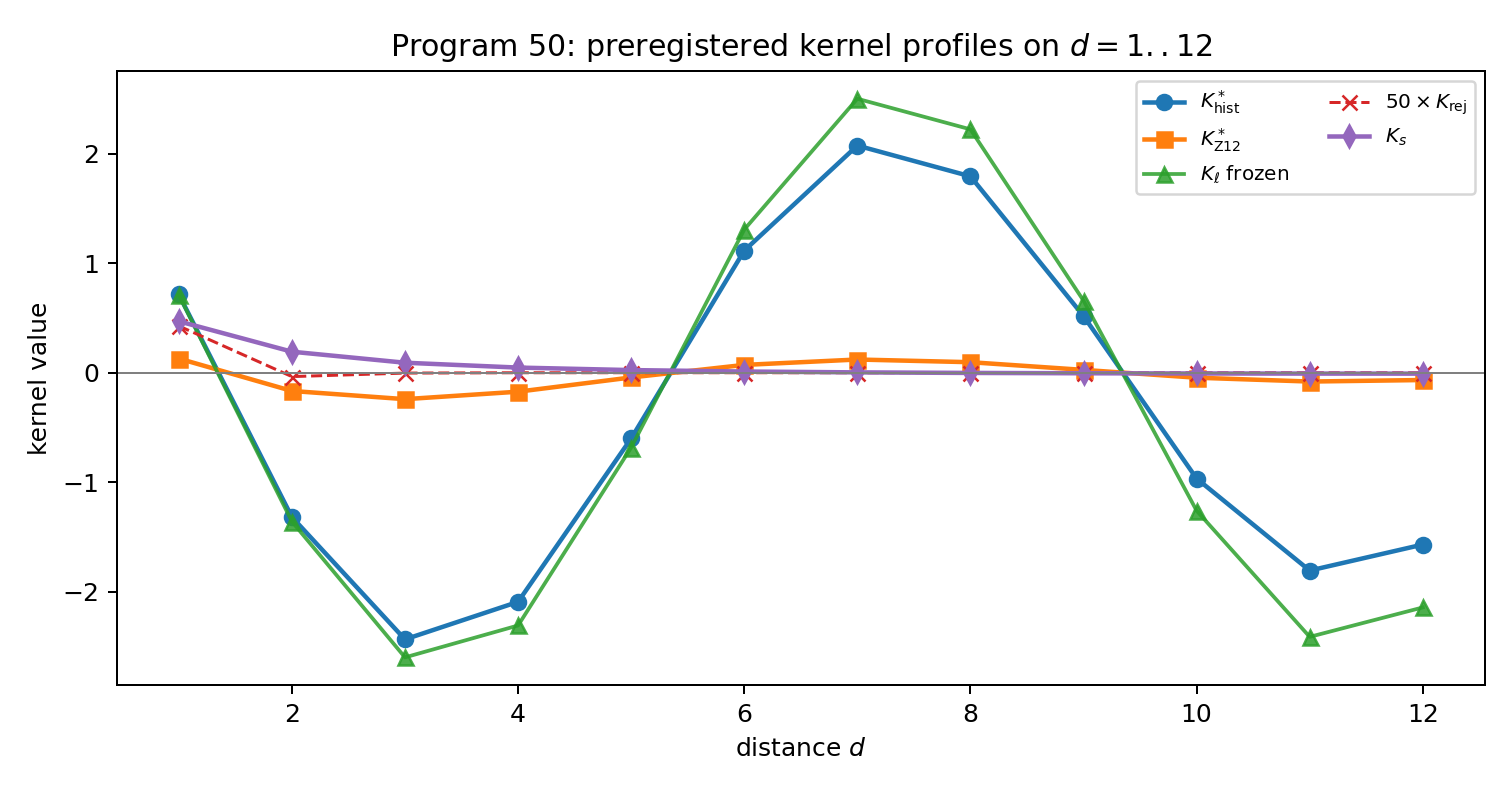
\includegraphics[width=0.92\textwidth]{FIN_Programs_41_50_Figures/program50_profiles.png}
\caption{Audited finite profiles. Visual proximity is not a derivation. The accepted scientific question is which typed map, if any, transports legacy data into strict data without importing the target.}
\end{figure}

\subsection{What ``twelve octaves'' currently means}

The rigorous carrier is $V=\Z/12\Z$, a circle of twelve labelled states with cyclic distance. Calling these states ``octaves'' is an interpretation. The old argument from the three-dimensional kissing number does not currently derive a physical energy-octave system.

Legacy* has exact carrier phase period eight, whereas the finite carrier has period twelve. Their combined repeat length is $\mathrm{lcm}(8,12)=24$. The legacy phase is not a character of $\Z_{12}$. This mismatch is not an inconsistency: it defines a sampled oscillatory profile, but it blocks a naive claim of exact twelve-octave phase closure. The strict phase is compatible with the finite circulant construction, and its spectral modes are the twelve Fourier characters of $\Z_{12}$.

The orientation pair $+\omega$ and $-\omega$ is isospectral. Chiral receivers and bispectral markers can detect a supplied orientation, but the radial kernel does not choose its sign. This is the live selector obstruction $QW\text{-}2191$.

\subsection{The status of the thirty fractal layers and Planck scale}

Historical documents proposed thirty layers, factors $\beta^N$, and a path from Planck to macroscopic scales. These claims were based on fitted hierarchies and weakly sourced physical identifications. Current work proves something narrower:

\begin{itemize}
\item repeated Schur elimination generates exact \emph{relative} scale ratios such as $2^k$; \proven
\item no dimensionless invariant can select an absolute length $\ell_*$, time $\tau_*$ or action $\hbar_*$; \proven
\item ``thirty layers'' is not derived by the strict operator or compression semigroup; \refuted\ as a present theorem
\item the Planck endpoint is an external dimensional anchor, not a strict internal unit; \proven\ as a provenance audit.
\end{itemize}

Accordingly, the compendium retains fractal layering as a future refinement hypothesis, but does not present thirty physical layers or the Planck scale as an achievement of FIN.

\section{The minimal finite mathematical core}

\subsection{Strict weights, generator and spectrum}

Let $d(x,y)=\min(|x-y|,12-|x-y|)$ on $\Z_{12}$ and set $W_{xx}=0$, $W_{xy}=K_{\rm strict}(d(x,y))$. The six positive off-diagonal weights are
\[
\begin{array}{lll}
k_1=0.46998567264502017,&k_2=0.19204355169010282,&k_3=0.09142861427792497,\\
k_4=0.04702916874565040,&k_5=0.02413122336363006,&k_6=0.011070817321442113.
\end{array}
\]
Every row has sum
\[
s=2\sum_{d=1}^{5}k_d+k_6=1.660307278766098953\ldots,
\qquad A=sI-W.
\]

\begin{theorem}[Strict Dirichlet identity]
For all $f\in\C^{12}$,
\[
\langle f,Af\rangle=\frac12\sum_{x,y}W_{xy}|f_x-f_y|^2\ge0.
\]
Since all off-diagonal weights are positive, $\ker A=\mathrm{span}\{\one\}$.
\end{theorem}

The Fourier modes diagonalize (A). Its audited spectrum is
\[
0,quad
0.754121154207080\ (\times2),\quad
1.577049514427610\ (\times2),\quad
1.961406861976446\ (\times2),
\]
\[
2.199568849333210\ (\times2),\quad
2.298606272079097\ (\times2),\quad
2.342182041146301.
\]
Thus the strict core has an exact finite graph-Laplacian interpretation. Calling (W) a physical interaction Hamiltonian, or (A) an energy, is an additional interpretation.

\subsection{One spectrum, two dynamics}

The same (A) gives
\[
\boxed{U_t=e^{-itA}},\qquad \boxed{P_t=e^{-tA}}.
\]
The first is a unitary group on amplitudes. The second is a positivity-preserving, uniform-reversible Markov semigroup on probability vectors. They share projectors and eigenvalues but not operational composition of observed probabilities.

\begin{table}[H]
\centering
\caption{The duality is spectral, not an identity of physical meanings.}
\begin{tabularx}{\textwidth}{@{}p{0.22\textwidth}XX@{}}
\toprule
Property & $U_t=e^{-itA}$ & $P_t=e^{-tA}$\\
\midrule
State object & complex amplitude / density operator after extra axioms & classical probability vector\\
Norm/invariant & Hilbert norm & total probability\\
Short-time escape & quadratic in (t) for position probabilities & linear in (t) when jumps are available\\
Interference & yes, after coherent preparation and amplitude measurement & no amplitude interference\\
Long-time behavior & quasiperiodic in finite dimension & converges to uniform equilibrium\\
Observed transition law & Born matrix generally not a semigroup & Chapman--Kolmogorov semigroup\\
Physical clock & not supplied by (A) & not supplied by (A)\\
\bottomrule
\end{tabularx}
\end{table}

\begin{figure}[H]
\centering
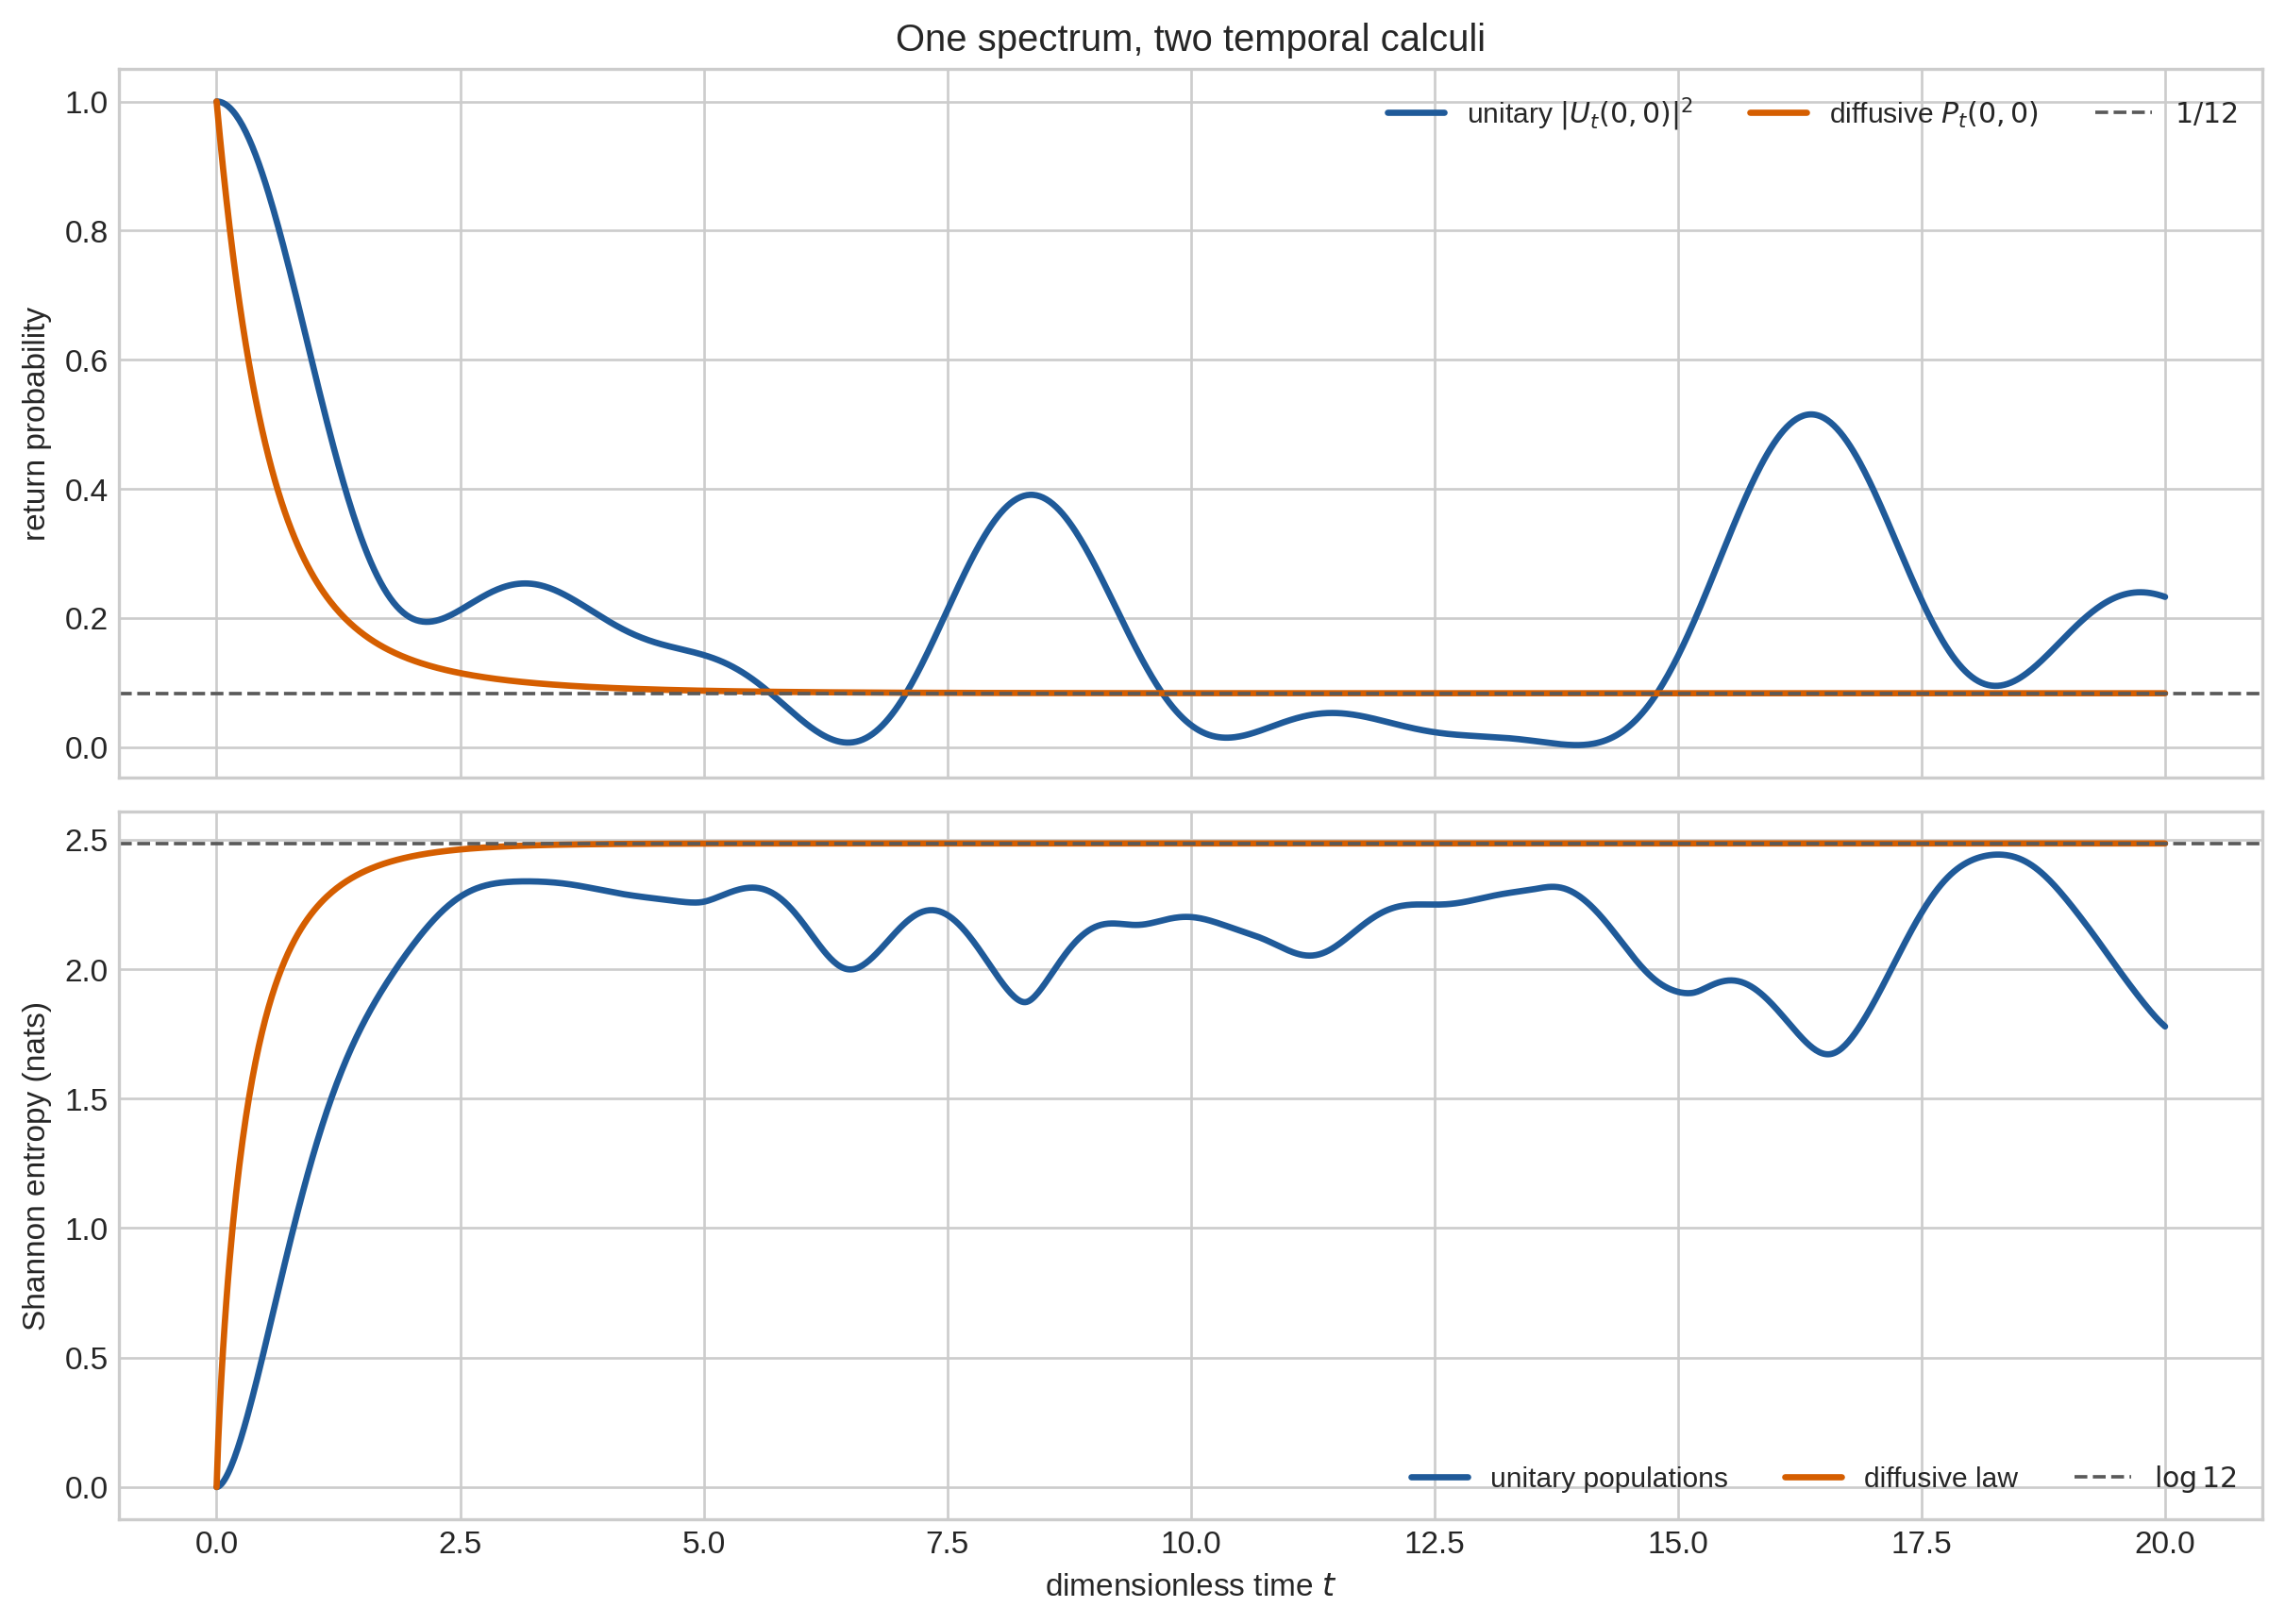
\includegraphics[width=0.88\textwidth]{FIN_One_Spectrum_Two_Dynamics.png}
\caption{The strict spectrum supports coherent and diffusive temporal calculi. The choice between them, or an open-system interpolation, requires an operational model.}
\end{figure}

This duality is one of FIN's clearest achievements. It also explains the observer paradox: an internal observer who has access only to populations may mistake dephased or coarse-grained unitary motion for diffusion. Distinguishing the models requires phase-sensitive preparations, multitime interventions and recorded outcomes.

\subsection{Green response and the common spectral object}

For $z\notin\sigma(A)$,
\[
G(z)=(zI-A)^{-1}=\int\frac{1}{z-\lambda}\,dE_A(\lambda).
\]
The same projector-valued measure $E_A$ generates $G(z)$, $U_t$, $P_t$, spectral filters and source response. This is the precise sense in which many repository structures are shadows of one object.

The Green resolvent also supports a corrected field-theoretic reconstruction. Given a supplied positive $L+m^2I$,
\[
S[\phi,K]=\frac12\phi^{T}(L+m^2I)\phi-J^T\phi+\Tr V(K)-\Tr(KC)
\]
has stationary equation
\[
(L+m^2I)\phi=J,\qquad \phi=(L+m^2I)^{-1}J.
\]
This reconstructs a minimal quadratic action from a propagator. If (V'(K)=C), it also gives a conditional operator potential. However, fitting (V) after observing a target (K) is always possible by finite polynomial interpolation and has no predictive force. The action is therefore a valid inverse construction, not yet a uniquely FIN-sourced fundamental Lagrangian.

Some earlier referee language classified strict as a normal-ordered screened discrete Green/Yukawa-type object. The robust surviving statement is the finite resolvent/Green interpretation. A unique continuum Yukawa field, metric, source law and renormalization prescription have not been derived.

\section{Fractal compression, memory and the observer}

\subsection{Exact Green--Schur compression}

Partitioning visible (E) and hidden (H) states gives the frequency-dependent effective operator
\[
A_{\rm eff}(z)=A_{EE}-A_{EH}(zI+A_{HH})^{-1}A_{HE},
\]
with self-energy
\[
\Sigma_E(z)=A_{EH}(zI+A_{HH})^{-1}A_{HE}.
\]
At zero frequency this reduces to the Schur complement. Eliminating alternating vertices in the tested $24\to12$ construction preserved retained Green response to residual $1.44\times10^{-14}$. This is an exact finite compression theorem, not a visual analogy.

\begin{figure}[H]
\centering
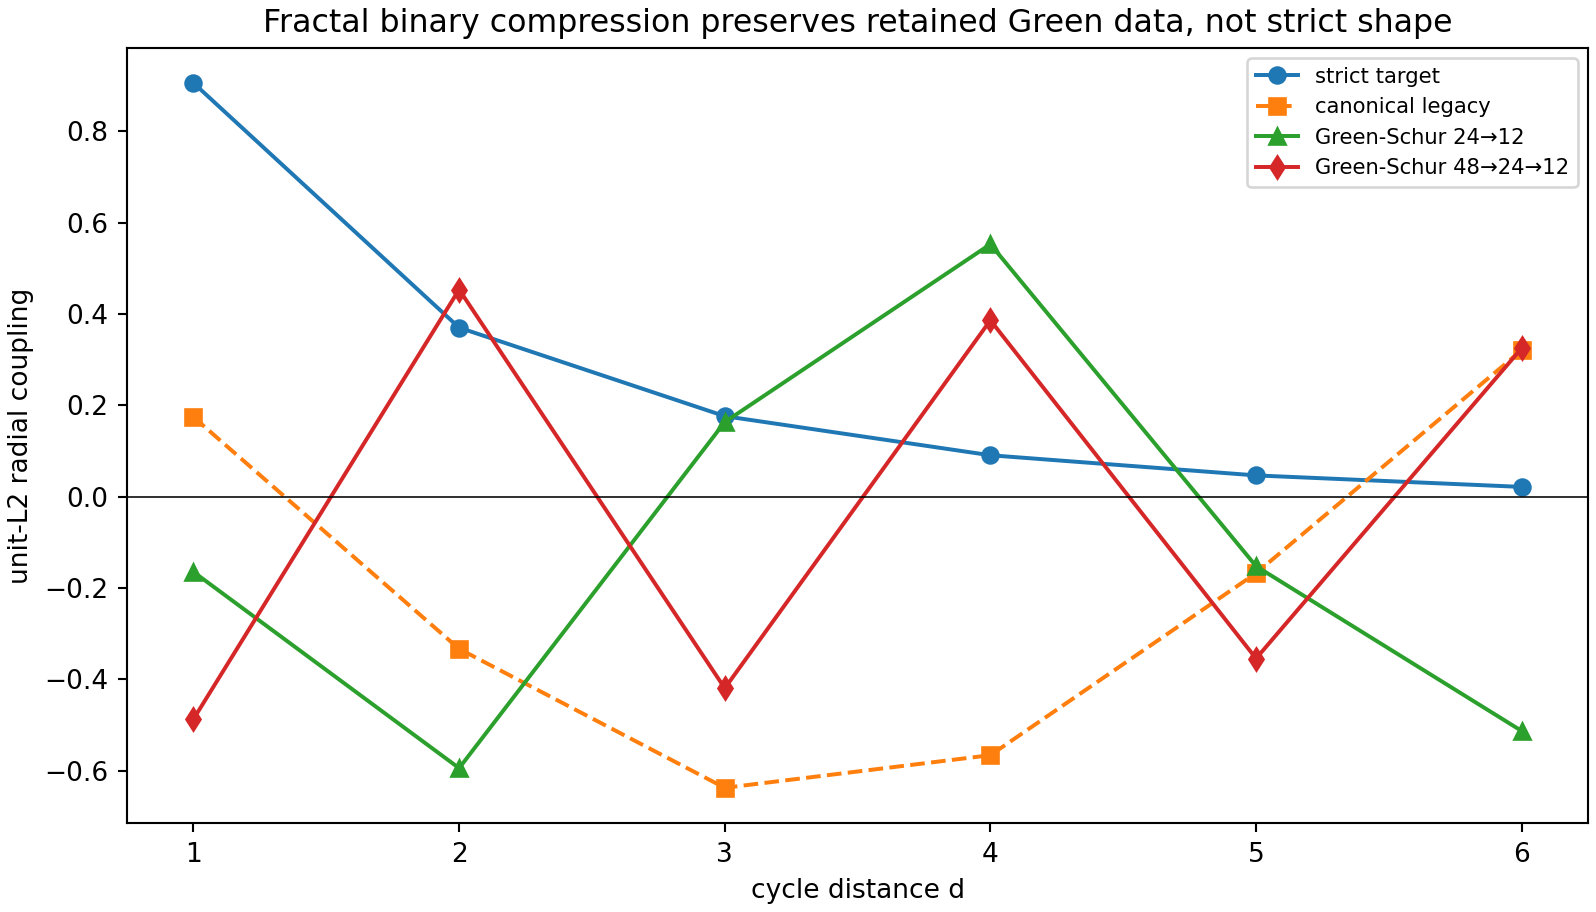
\includegraphics[width=0.88\textwidth]{FIN_Programs_51_60_Green_Fractal_Physics_Figures/program55_fractal_compression.png}
\caption{Exact response-preserving elimination generates a hierarchy of effective descriptions. It gives relative scale and hidden-state memory, but did not generate the strict kernel in the executed tests.}
\end{figure}

The dynamic self-energy is a Stieltjes-type matrix function. Its time transform is a memory kernel, connecting Green functions, Mori--Zwanzig/Feshbach reduction, adaptive reservoirs and contextual observation. The second-generation atlas identified the \emph{Stieltjes--Schur Context Functor} as the most informative derived object:
\[
\text{Green response}\leftrightarrow\text{compression}\leftrightarrow
\text{memory}\leftrightarrow\text{observer context}\leftrightarrow
\text{accessible information}.
\]

\subsection{What compression explains and what it does not}

Compression explains how hidden degrees of freedom modify visible laws, create nonlocal memory and reduce distinguishability. In a regularized Gaussian information model, the legacy-versus-strict divergence fell from (23.63624) to (11.60157), consistent with data processing. This is apparent information loss from the retained context, not ontological deletion.

Compression did \emph{not} produce $\eta=1.8$, the strict phase, a physical length or the missing orientation sign. Its exact achievements are therefore substantial but bounded:

\begin{itemize}
\item exact marginal response and composable coarse graining: \proven;
\item dynamic memory/self-energy space: \proven;
\item a nontrivial fractal fixed point in that function space: \speculative;
\item strict as a static fixed point of binary compression: \refuted\ in the tested family;
\item absolute physical scale from fractal ratios: \refuted.
\end{itemize}

\subsection{Information loss, negative coupling and signed resources}

The phrase ``negative information coupling'' admits at least three inequivalent meanings:

\begin{enumerate}
\item a negative scalar kernel entry;
\item contraction of accessible distinguishability after a channel or context restriction;
\item signed mass needed to represent a target attenuation as a mixture of simpler paths.
\end{enumerate}

Only the second is automatically an information-theoretic loss. The executed programs proved that a larger reversible description can retain information that disappears from the observed subsystem. The raw signed legacy operator is not a Markov generator; absolute-value, positive-part or conservative-shift repairs must be declared.

For the strict attenuation sequence $h_k=(1+k^{9/5})^{-1}$, every positive exponential-distance mixture obeys Hausdorff moment inequalities, but $\Delta^4 h_0=-0.0715275581$. A signed representation is therefore necessary. The exact seven-moment minimum negative Jordan mass is
\[
\mathcal N_{\rm path}^{\min}=0.406706334692258\ldots,
\]
with a certified interval lower endpoint (0.4067063265581317). For the full oscillatory twelve-moment profile the later exact enclosure was narrowed to approximately
\[
0.7073534379053974\le\mathcal N_{\rm osc}\le0.7073534683998260.
\]
These are rigorous classical signed-representation costs. They are not negative energy, quantum negativity, information destruction or laboratory loss.

\section{Phase coherence, symmetry and the missing selector}

\subsection{What phase results are established}

The project contains several genuine phase results:

\begin{itemize}
\item the legacy phase $\pi d/4+\pi/6$ is exact and has period eight in its carrier;
\item the strict frozen decimals are generated by the procedural lattice $1/4000$, with $0.18575=743/4000$ and $0.16250=13/80$;
\item finite Fourier projectors give exact modal coherence on $\Z_{12}$;
\item chiral bispectra and inversion-odd receivers distinguish a supplied (+/-) sector;
\item Schur compression transports the chiral receiver while preserving the mirror relation.
\end{itemize}

The $1/4000$ unit has scan/refreeze provenance. It is not an internally derived physical phase quantum. The exact identity $\alpha_{\rm geo}=4\ln2=\ln16$ and
\[
A_\phi=\frac{2\pi}{\alpha_{\rm geo}}=\frac{\pi}{2\ln2},\qquad
\alpha_{\rm geo}A_\phi=2\pi,
\]
is mathematically exact. Since $\alpha_{\rm geo}/(2\pi)$ is irrational, it does not yield a finite cyclic clock or a canonical orientation.

\subsection{Why mirror symmetry is not broken internally}

On a radial $\Z_{12}$ kernel, inversion $d\mapsto-d$ leaves the spectrum unchanged. Exhaustive audits of automorphism-invariant Boolean predicates and orbit-constant scoring functionals failed to distinguish $+1$ from $-1$. This is not a lack of cleverness but a no-section obstruction: an invariant object cannot canonically choose between symmetry-related branches.

An apparatus orientation, boundary condition, chiral state or perturbation can select a branch. That is a valid \conditional{} physical model. It is not a strict-core derivation. Consequently no current result discharges $QW\text{-}2191$, and no old oriented physical role may be transferred from legacy to strict without a separate role-transfer theorem.

\section{Shannon information and the bridge to thermodynamics}

\subsection{What the four-bit identity proves}

For a uniform sixteen-state source,
\[
H=\ln16=4\ln2=\alpha_{\rm geo}.
\]
This is exactly four bits in natural logarithmic units. It gives a compact informational normalization candidate and explains why $4\ln2$ recurs in the legacy programme. It does not uniquely determine a kernel amplitude, a physical entropy or a mass.

For any stochastic channel $T$, relative entropy satisfies data processing,
\[
D(p\|q)\ge D(Tp\|Tq).
\]
This is the rigorous foundation for the FIN accessible-information ledger. Unitary position probabilities can exhibit information backflow because the population map is not a Markov semigroup; the executed strict/Legacy* tests found monotone Markov information and numerous unitary Born backflow steps.

\subsection{Why information is not yet energy}

Every strictly positive finite probability vector can be written as a Gibbs distribution at infinitely many energy scales:
\[
E_i=-\theta\log p_i+C,\qquad \beta=\theta^{-1}.
\]
Changing $\theta$ changes all energy gaps while preserving $p$. A modular Hamiltonian $-\log\rho$ is likewise dimensionless until time or temperature is calibrated. Landauer's equality can be reproduced after a Hamiltonian, bath, temperature and erasure process are supplied; it does not assign energy to a bit in isolation.

The minimal conditional thermodynamic bridge is therefore a tuple containing at least a state, Hamiltonian, inverse temperature, allowed processes and an energy/action calibration. FIN currently supplies the informational side of this bridge, not its physical scale.

\section{Can the soliton's frequency generate time?}

The intuition that a persistent oscillation carries time is scientifically useful. Mathematically, a nonzero spectral gap $\widehat\omega$ supplies a dimensionless phase parameter
\[
\varphi(t)=\widehat\omega t\pmod{2\pi}.
\]
If a mode is persistent and observable, its phase can define an \emph{internal relational clock}: other processes can be compared with its cycles. Ratios $\widehat\omega_i/\widehat\omega_j$ and cycle counts are intrinsic.

Three steps remain external:

\begin{enumerate}
\item choose which dynamics and which mode is the clock;
\item prove persistence, readability and sufficiently small drift under the declared environment;
\item calibrate one cycle against a physical second, or supply an equivalent dimensional reference.
\end{enumerate}

Rescaling $t\mapsto ct$, $A\mapsto A/c$ preserves all dimensionless phase relations. Therefore the spectrum can generate order, periodicity and relative duration but not an absolute second. The user's intuition is best promoted to the following local research conjecture:

\claimbox{\textbf{Relational clock conjecture.} A persistent nadsoliton mode plus an operational record functor can define an internally observable time coordinate up to positive affine rescaling. Absolute time units remain a calibration resource.}

This conjecture is compatible with the current obstruction and can be investigated without claiming that time in nature has already been derived.

\section{Matter, light and old physical-role claims}

\subsection{The historical emergence picture}

The founding programme proposed that particles are stable topological defects or self-sustaining informational domains, that mass measures the cost of changing such a pattern, and that light and matter arise as modes of one field. This is a coherent research narrative. It resembles nonlinear field defects, Hopfions, information-processing cost and emergent quasiparticles.

However, the current finite kernel does not provide the mathematical objects required to make those identifications unique: a continuum/refinement space, a nonlinear field equation, boundary conditions, a topological charge, gauge group and representations, spin/statistics, dimensional action and a calibrated observable map. A finite twelve-state radial matrix alone cannot prove that one eigenmode is an electron or that a winding number is a particle generation.

\subsection{Audit of the principal historical physical claims}

\begin{longtable}{@{}p{0.30\textwidth}p{0.22\textwidth}p{0.38\textwidth}@{}}
\caption{Status of historical physics claims.}\\
\toprule
Claim & Current status & Reason\\
\midrule
\endfirsthead
\toprule
Claim & Current status & Reason\\
\midrule
\endhead
Particles are topological defects of the nadsoliton & \speculative & No strict continuum field, defect class or stability theorem connects the finite kernel to particles.\\
Mass $=$ topology $\times$ resonance / processing intensity & \speculative & Historical correlations and fitted formulas are not a noncircular derivation; the mass unit and topological assignment are missing.\\
Four-bit jumps explain lepton/proton masses & \refuted\ as a derivation & Approximate post-hoc fits and ad hoc assignments do not identify unique particle sectors or held-out predictions.\\
\(\sin^2\theta_W=\alpha_{\rm geo}/12\) & heuristic only & The formula is not a proved operator functional and has no strict role-transfer certificate.\\
\(\alpha_{\rm EM}^{-1}=\alpha_{\rm geo}(1-\beta_{\rm tors})/(2\beta_{\rm tors})\) & model-level / conditional & It depends on a historical parameter coordinate and fails the required gauge/role-transfer test.\\
Gravity hierarchy $\beta^N$ and thirty layers & \speculative / downgraded & A dimensionless fitted hierarchy does not create Newton's constant, Planck length or a sourced layer number.\\
Strict kernel gives Standard Model, GR or quantum gravity & \refuted\ as a present claim & Gauge, spin, Lorentzian, metric, stress--energy, continuum and unit structures are absent.\\
Nadsoliton $\to$ light $\to$ matter $\to$ observer & ontology/program order & It remains the preferred FIN emergence programme, not a completed derivation.\\
\bottomrule
\end{longtable}

The honest answer to whether the old matter programme ``had any sense'' is therefore twofold. It had legitimate heuristic value: stable modes, nonlinear defects and internal observers are standard mathematical mechanisms worth testing. Its specific particle identifications and mass formulas do not survive as established results. This compendium retains the research questions and rejects their promotion to physics.

\section{The missing physical structure}

\subsection{Why the operator is not a complete theory}

A self-adjoint matrix does not specify what is prepared, how time is calibrated, what is measured, which environment is ignored, what apparatus defines orientation, or what event becomes a record. The smallest current architecture is
\[
\boxed{W_0+\mathrm{CA}+\mathrm{OA}\quad(+\mathrm{SA}\text{ when orientation matters})}.
\]

Here:

\begin{itemize}
\item $W_0$: the dimensionless informational core --- carrier, kernels with distinct roles, $A$, spectral measure, Green response, compression and information geometry;
\item CA: conversion axioms, minimally a basis equivalent to $(\ell_*,\tau_*,\hbar_*)$;
\item OA: operational axioms
\[
(\rho_0,\mathcal P,\mathcal T,\mathcal I,\mathcal E,\mathcal A,\mathcal R),
\]
for state, preparation, dynamics/clock, instrument, environment, apparatus and record;
\item SA: a reference origin/orientation/chirality and its coupling law when the outcome is sign-sensitive.
\end{itemize}

The rank-three unit basis is necessary because independent rescalings of length, time and action leave the dimensionless FIN core invariant. Removing one leaves at least one of length, time, energy, mass or action underdetermined.

\subsection{Operational completion by processes and testers}

Process tensors/quantum combs provide the most developed mathematical home for the missing observer structure. A comb represents multitime dynamics with memory; a tester represents allowed preparations and instruments; classical outcome registers represent records. Clock and reference calibration determine how the abstract slots map to laboratory operations. This framework can distinguish coherent, Markov, dephasing and non-Markovian descriptions of the same spatial operator.

It does not create a unique apparatus from the kernel. It tells us how to state and falsify one proposed apparatus. This is exactly the boundary between a mathematical model and empirical physics.

\section{The constructed experiment and executable specification}

FIN Release 10.21 constructed a transfer package rather than claiming an experiment had occurred. Its five compulsory measurement obligations are:

\begin{enumerate}
\item basis and informationally complete preparations;
\item a calibrated time variable;
\item a vertex-resolving POVM;
\item finite event-level transition counts;
\item an independent record, frozen hold-out and separation of provider, registrar and analyst.
\end{enumerate}

The first four can be specified and validated by mathematics/software. The fifth cannot be generated by code in the same custody chain.

\subsection{P240--P242}

\begin{itemize}
\item \textbf{P240} freezes a twelve-state heat-kernel tomography design. Its optimal dimensionless acquisition time is $\tau_*=1/\lambda_{\max}\approx0.426952$, with allocation and finite-shot guidance.
\item \textbf{P241} is a fail-closed validator for preparations, clock, vertex measurement, event data, hashes and custody roles.
\item \textbf{P242} is a one-shot held-out pipeline for semigroup and projective-spectrum tests. It may not run before the external gate passes and must report failure without repairing the model after unblinding.
\end{itemize}

\begin{figure}[H]
\centering
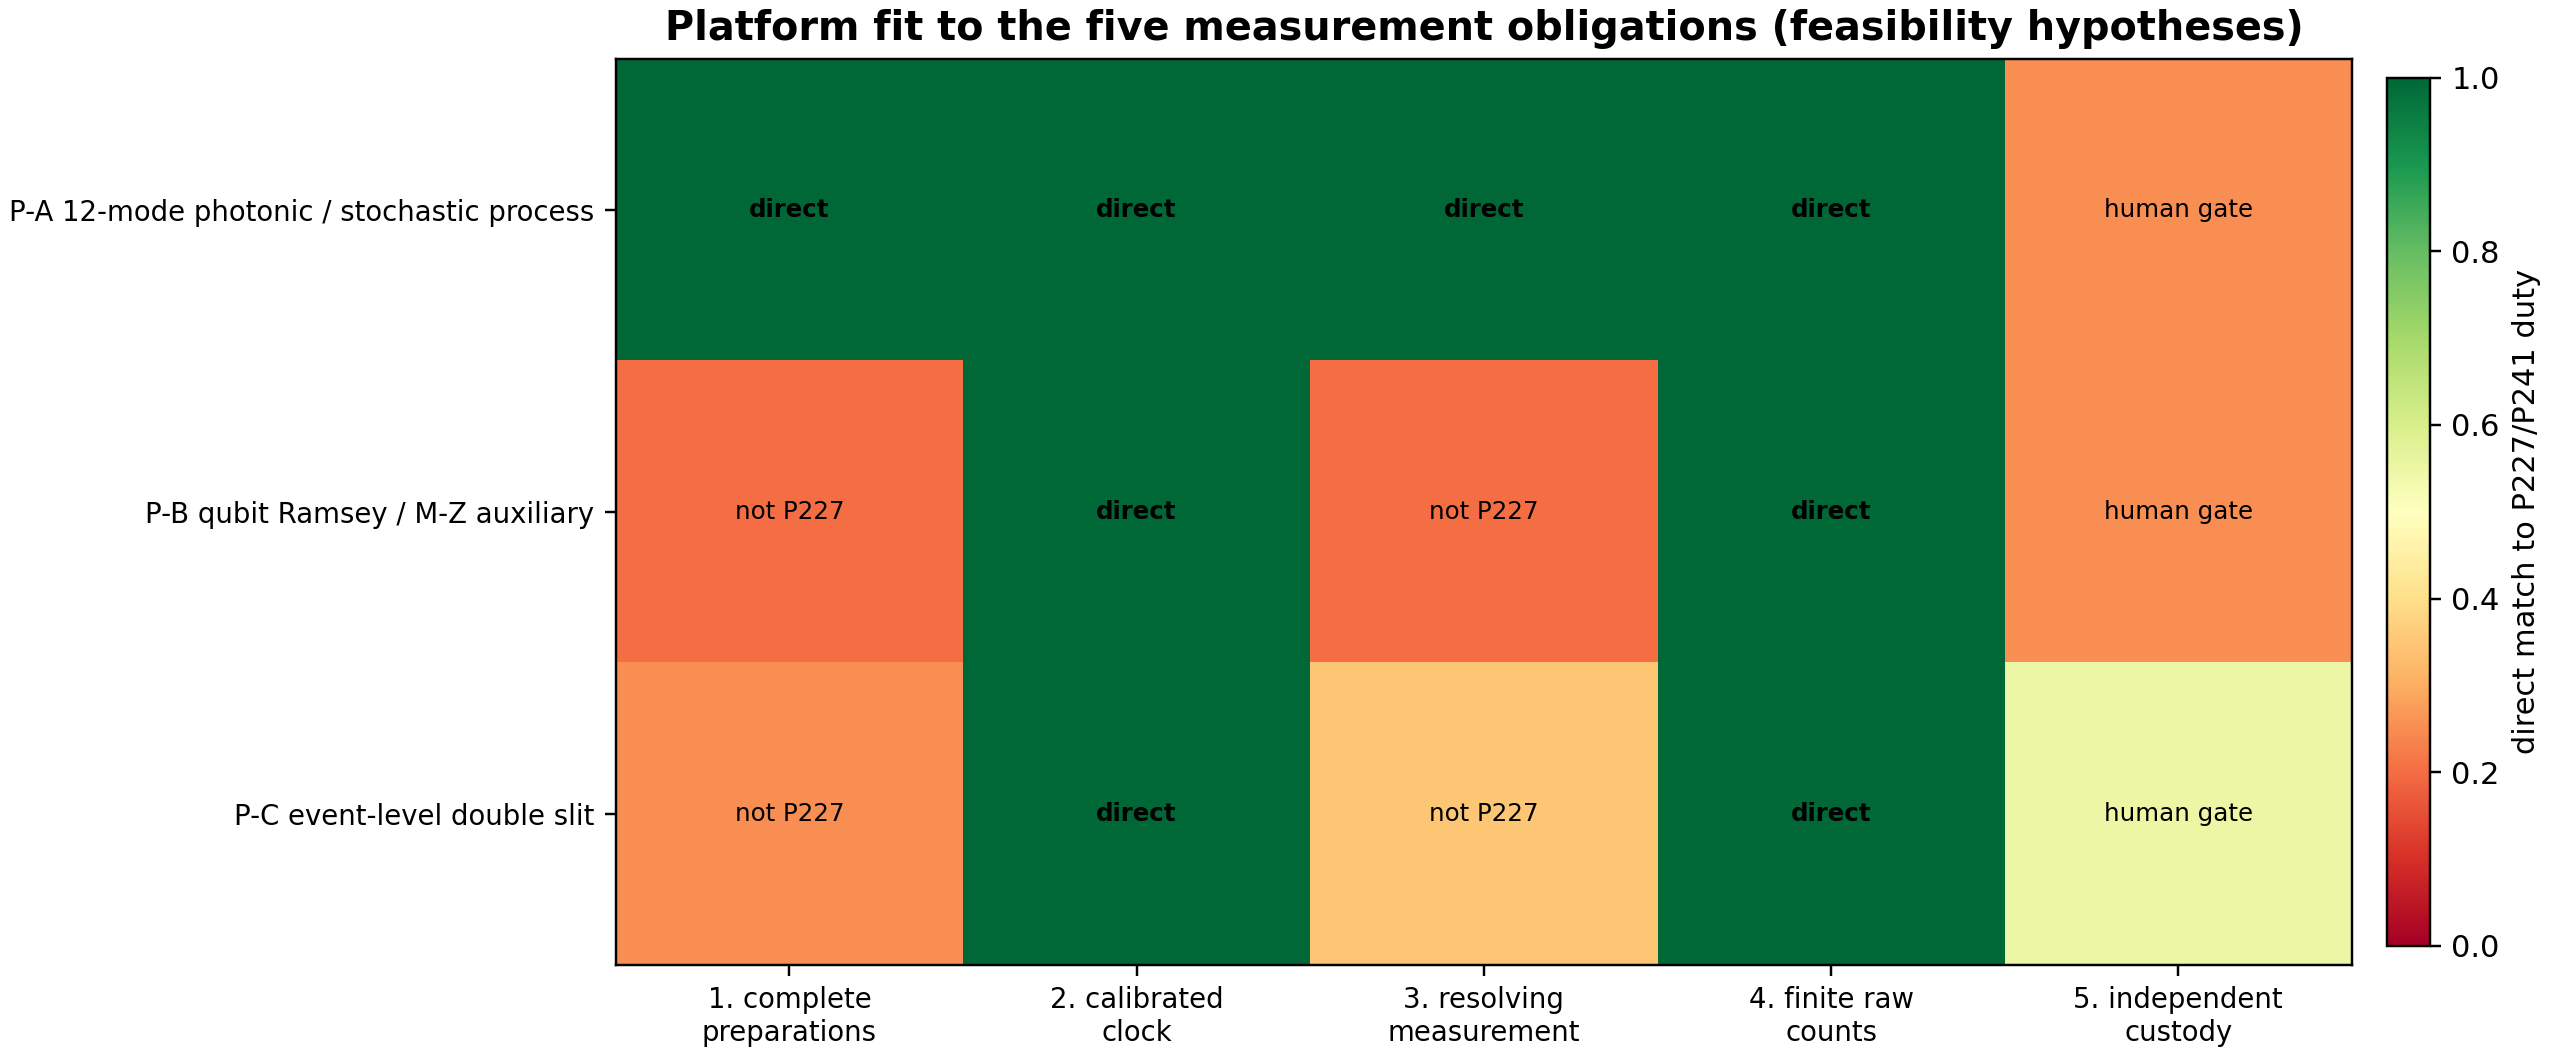
\includegraphics[width=0.94\textwidth]{FIN_Lab_P240_242_Transfer_Figures/platform_obligation_matrix.png}
\caption{The operational obligation matrix. This is an executable specification of what a physical test must supply, not evidence that the apparatus exists.}
\end{figure}

\subsection{Candidate platforms}

The primary feasibility hypothesis is a photonic continuous-time walk on a twelve-mode graph, with single-photon or weak coherent preparation, an interferometric/waveguide implementation, controlled dephasing/loss, vertex-resolving detectors and time-tagged events. An interferometric qubit/Ramsey platform is an auxiliary coherent/dephasing test. An event-level double slit is a custody and coherence control and must store raw tuples $(t,x,y,\mathrm{configuration},\mathrm{run\ id})$, not only an image.

\begin{figure}[H]
\centering
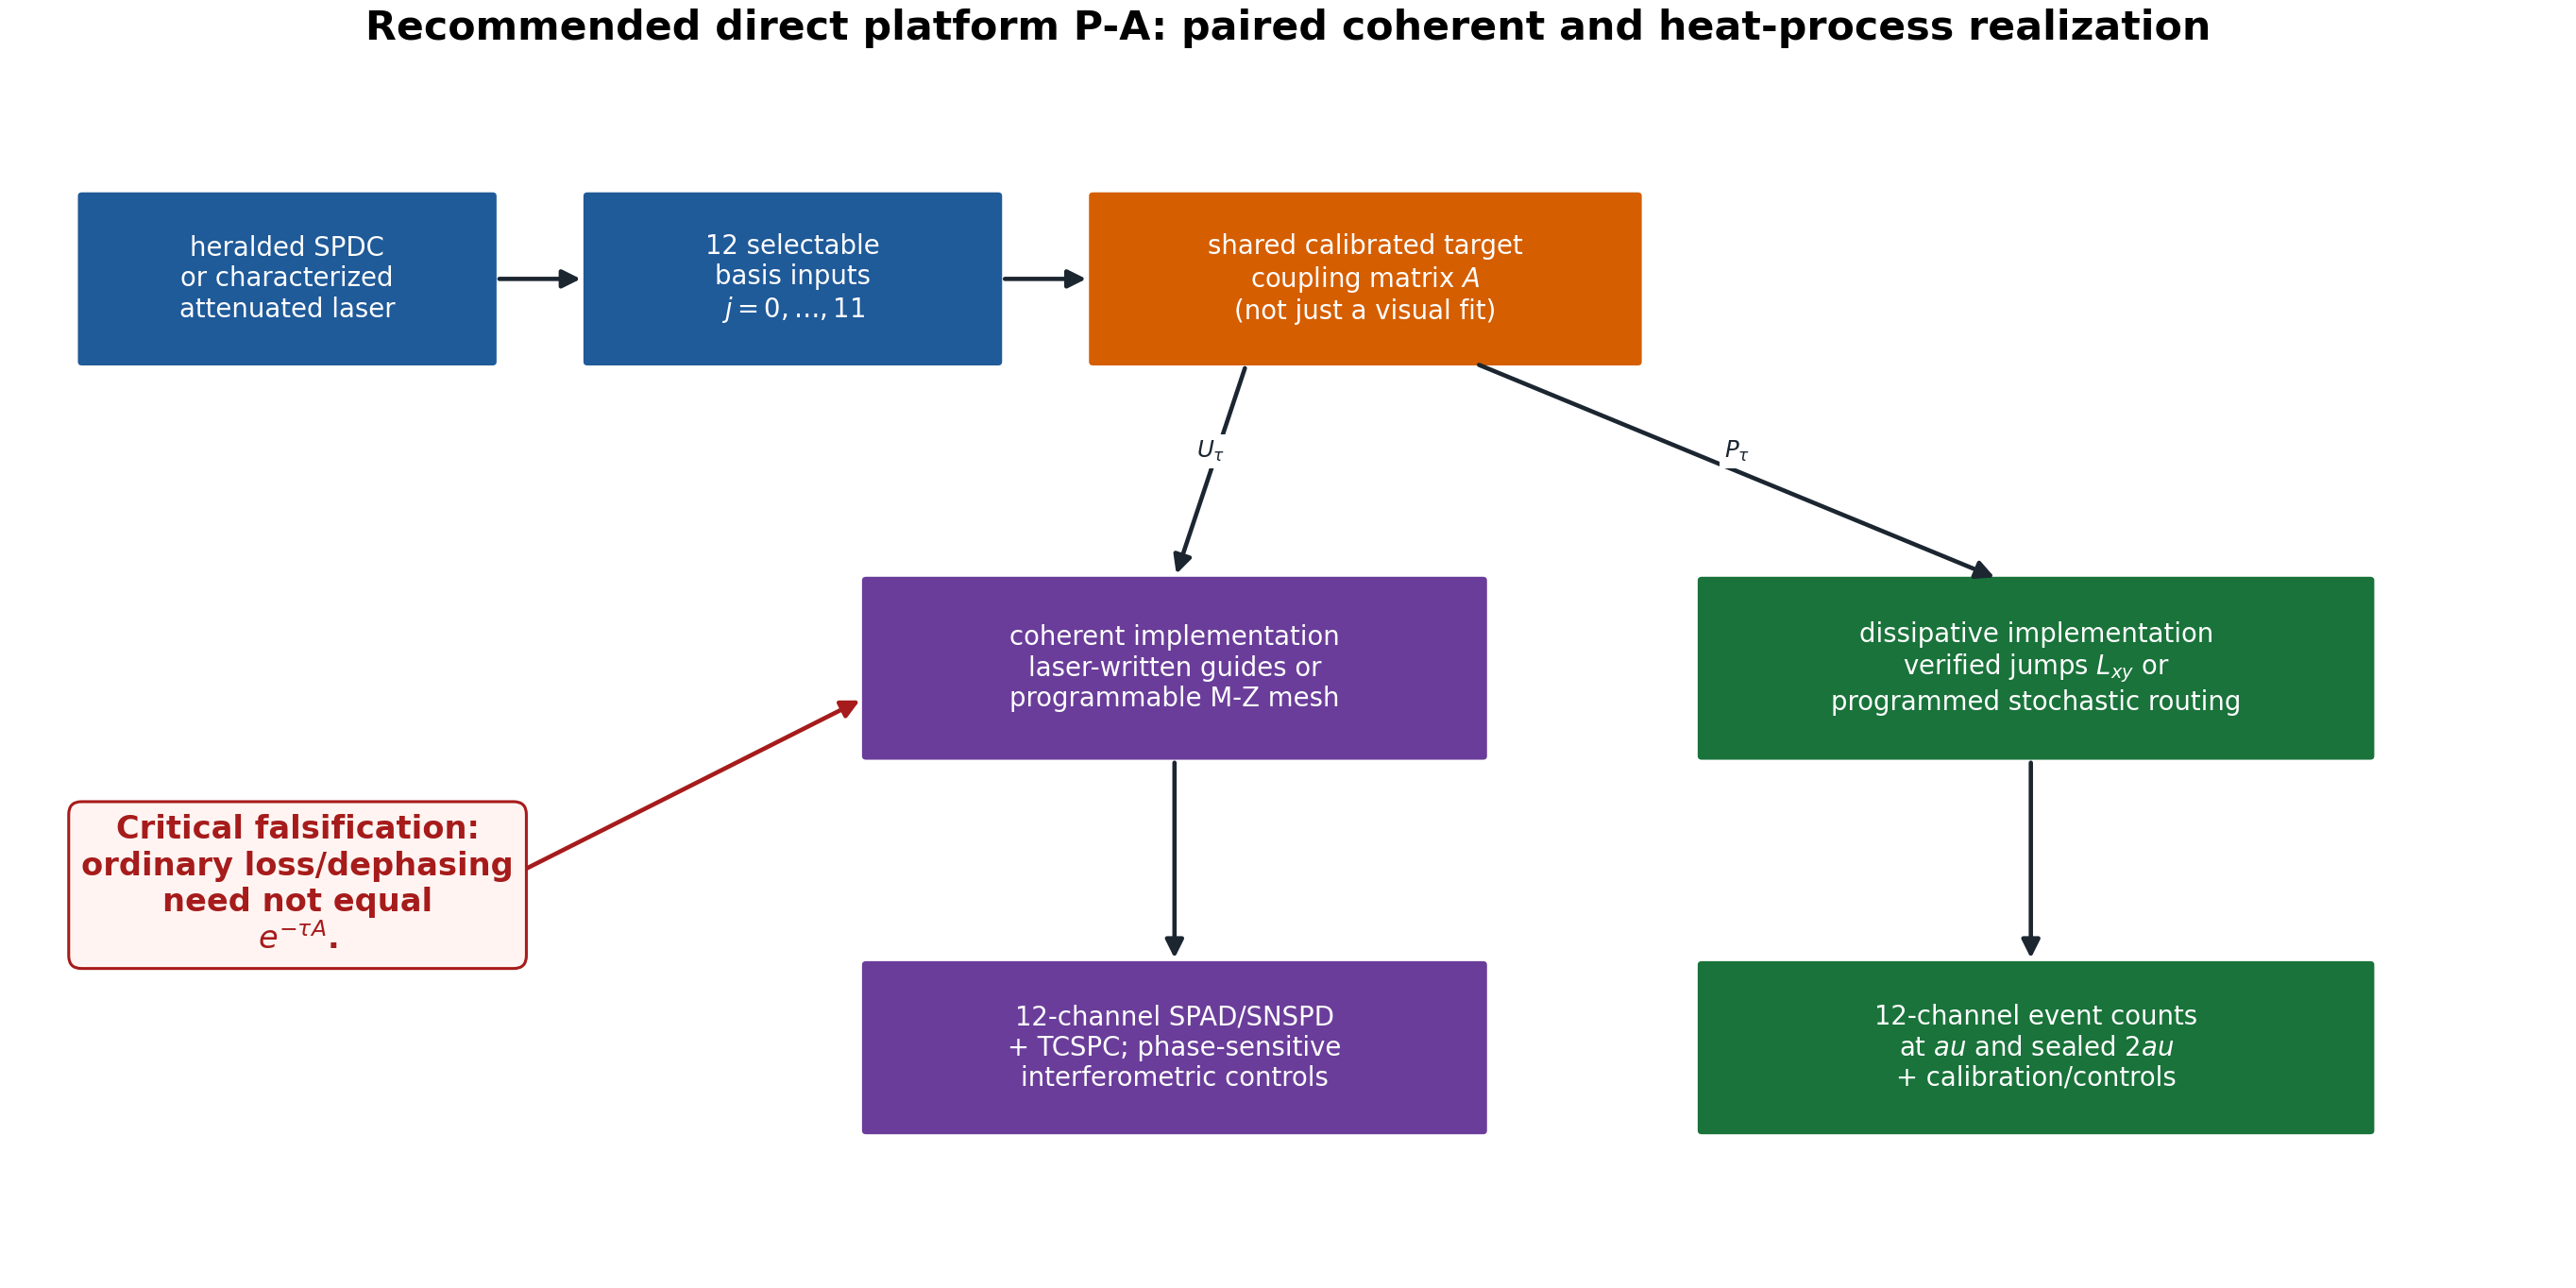
\includegraphics[width=0.90\textwidth]{FIN_Lab_P240_242_Transfer_Figures/platform_A_apparatus.png}
\caption{Candidate twelve-mode photonic realization. Every arrow is a hypothesis to be certified by experimental physicists.}
\end{figure}

The finite double-slit model predicts an interference cross term for coherent two-vertex preparation and its suppression by a which-path record. It is a valid finite operational analogue, not a simulation of continuum optical diffraction and not by itself a test of the twelve-state heat semigroup.

\begin{figure}[H]
\centering
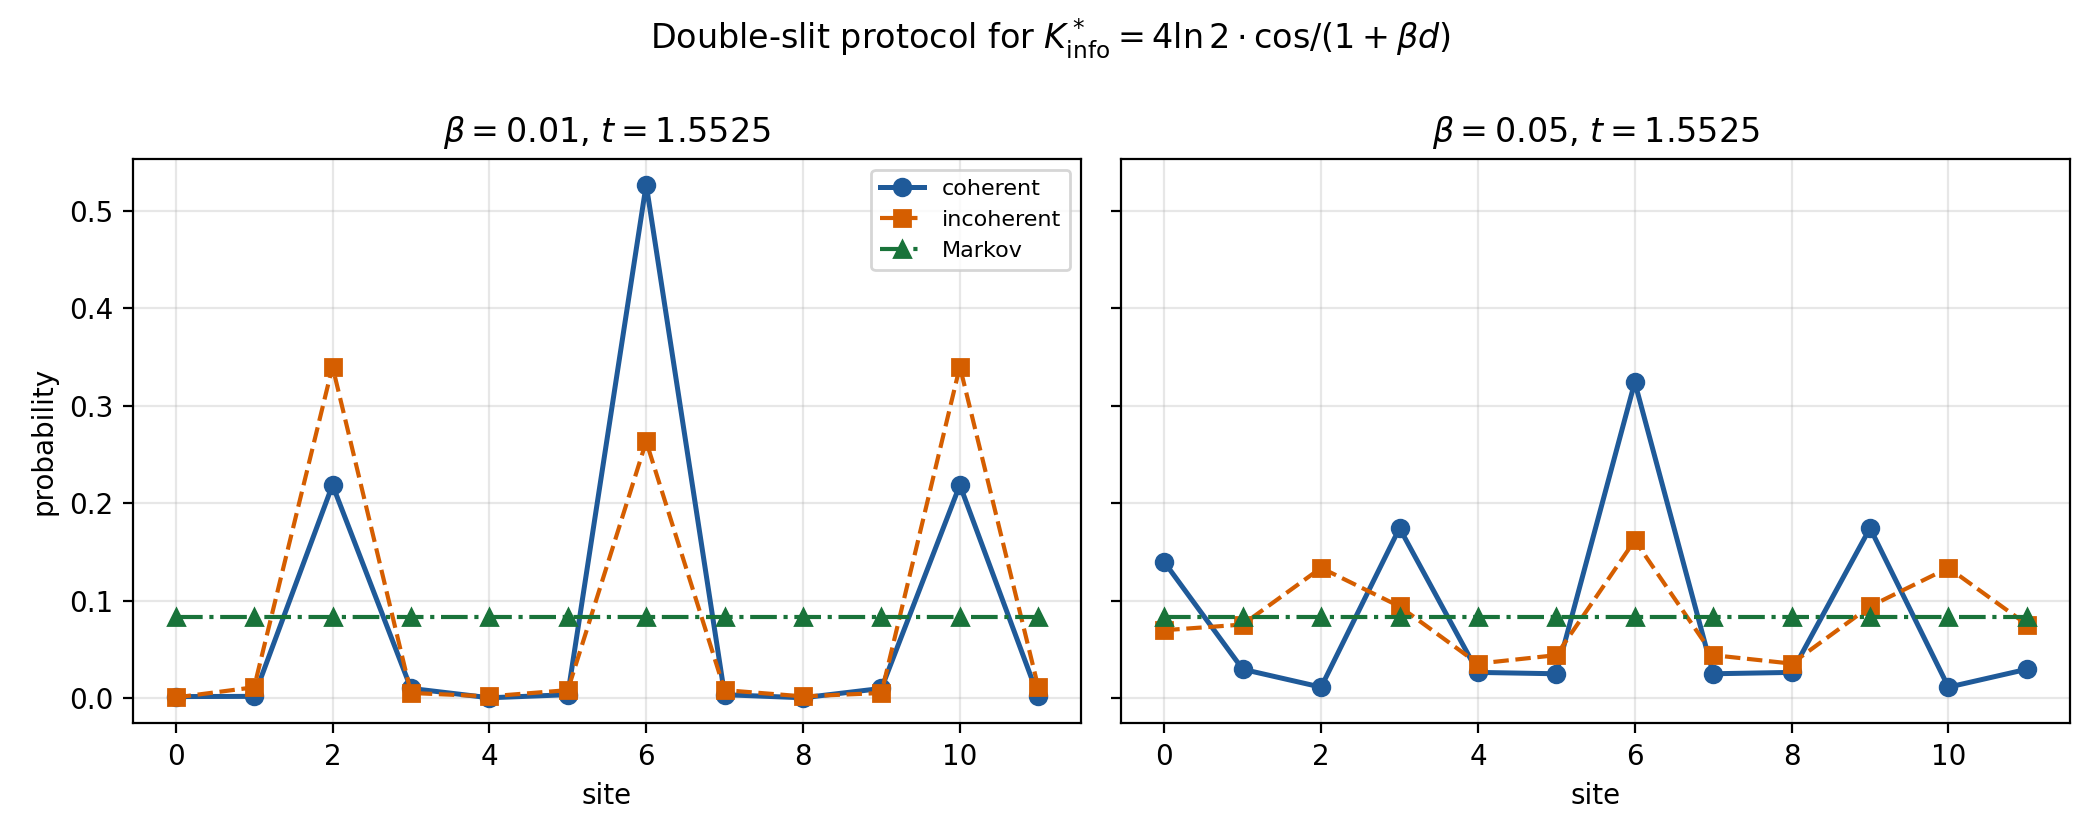
\includegraphics[width=0.90\textwidth]{FIN_KStar_Info_4ln2_Figures/double_slit.png}
\caption{Finite event-model double-slit comparison. The figure illustrates a model-discrimination observable; it is not laboratory data.}
\end{figure}

No external bundle has passed P241. Hence the current statement is: \conditional\ a falsifiable experiment has been designed; \refuted\ the claim that FIN is already laboratory validated.

\section{Later research: signed resources and exact operational mathematics}

\subsection{From P295 to P393}

Later local programmes sharpened the legacy--strict boundary and the operational interface:

\begin{itemize}
\item strict attenuation cannot be a positive fixed-phase mixture of legacy exponential paths; exact signed-resource lower bounds were certified;
\item the legacy finite phase group and strict procedural nontorsion phase resource cannot be connected by a torsion-preserving map;
\item scalar finite interpolants can map one $C_{12}$ spectrum to another but fail transfer to other carriers, proving interpolation is not universality;
\item a six-outcome informationally complete finite POVM, loss-aware synthetic photonic model and multitime testers were constructed;
\item FIN Operational Resource Completion (FORC) typed the missing preparation, time, measurement, environment and record resources;
\item exact operational realizations of signed sampling were constructed with ordinary probabilities and a sign register, without interpreting the signed measure as negative physical probability;
\item no independent hold-out, calibrated hardware, physical reservoir or dimensional standard was admitted.
\end{itemize}

These results make the framework more falsifiable and reproducible. They do not complete the physical bridge.

\subsection{The P394--P486 exact causal-tester frontier}

The most advanced current local mathematics concerns reduced multitime phase/dephasing discrimination. It is downstream of the FIN operator and should not be mistaken for a kernel derivation.

\begin{itemize}
\item P451 proved a coherent tester advantage over the complete diagonal face.
\item P454--P469 reduced a global primal--dual gap through exact nested dual certificates and support/KKT structure.
\item P471--P473 reduced the support condition to thirteen cubic polynomial orbits, proved a strict rational Krawczyk inclusion and positivity, and certified exact global attainment of one O167 optimizer for the declared reduced three-slot problem. The value lies in
\[
[0.5233281002710117,\ 0.5233281002710717].
\]
\item P483 proved persistence in a small parameter rectangle. Root uniqueness is local to the certified box.
\item P474/P484 found strong evidence for a complex optimal-face direction but also an exact counterexample showing that Riccati congruence and orientation alone do not force the missing causal axis. Full-cone nonuniqueness remains open.
\item P480 independently replayed the exact interval certificate with the Python standard library.
\item P486 certified determinant signs, the positive standard branch, a nonzero pivot and $\det(B_{\rm map})=+1$. It did not prove the causal equal-endpoint identity.
\end{itemize}

This is genuine computer-assisted mathematics. It supplies no selector, unit, laboratory record, legacy-to-strict completion, particle theory or gravity.

\section{The twenty-hour Singular/Kaggle checkpoint}

The supplied archive \texttt{FIN\_Singular\_Checkpoint\_after\_PREPARE.zip} was independently inspected for this compendium. Its SHA-256 is
\begin{center}
\small\texttt{a55500e30a194cb16ced94266c17e29e5b555669e064fcbda242c52a3f535a67}.
\end{center}

It contains an exact rational input object of about (12.7) MB, a manifest, a prepare-status file and campaign state. The decisive facts are:

\begin{itemize}
\item status: \texttt{prepared\_exact\_QQ\_system};
\item eleven reduced variables and eleven reduced generators;
\item five P485 target polynomials;
\item coefficient closure $\sqrt2=2-4\alpha^2$ for $\alpha=\sin(\pi/8)$;
\item no literal \texttt{sqrt} remains in the prepared rational system;
\item the recorded preparation stage took about (1170.72) seconds;
\item the largest generator has about (1.85) million characters;
\item no P485 Gröbner basis, no five normal-form remainders and no P487 elimination relation are included.
\end{itemize}

The checkpoint is therefore a valuable reproducible input artifact and proves that the earlier $\sqrt2\to\mathbb Q$ implementation defect was repaired at the preparation layer. It is not a P485 or P487 scientific verdict. The user's longer Kaggle wall time may include queueing or a later computation, but the archive itself certifies only PREPARE; this report does not infer missing results.

\section{What the theory now is --- and is not}

\subsection{The deepest surviving mathematical interpretation}

\claimbox{\textbf{Deepest surviving interpretation.} FIN is presently a finite, dimensionless spectral-information and contextual-operator framework. A self-adjoint generator and its spectral measure unify strict graph response, Green functions, unitary and diffusive dynamics, variational source response and exact contextual compression. Adaptive learning, orientation, units and physical observation require additional typed laws.}

This interpretation is stronger than saying the repository contains unrelated analogies. The Green/spectral/Schur identities are exact. It is also narrower than a field theory, neural universe or Theory of Everything. The current ranking is:

\begin{table}[H]
\centering
\caption{Quantitative interpretation ranking, 0--100, based on present theorem coverage.}
\begin{tabularx}{\textwidth}{@{}XccX@{}}
\toprule
Interpretation & Score & Confidence & Main limitation\\
\midrule
Finite spectral operator / graph signal framework & 94 & high & finite and dimensionless\\
Contextual Green--Schur information dynamics & 91 & high & context split is supplied\\
Operational process/tester research programme & 84 & high & no admitted laboratory record\\
Adaptive operator / inference engine & 68 & moderate & learning law is additional and not uniquely sourced\\
Information geometry & 65 & moderate & likelihood/state family and units are supplied inputs\\
Self-referential dynamical system & 60 & moderate & feedback integrability and selector remain open\\
Neural operator / reservoir model & 52 & moderate & analogy and conditional benchmarks, not ontology\\
Finite noncommutative geometry & 48 & moderate & many spectral triples fit the same finite data\\
Field theory & 34 & low & no continuum, metric family or complete action\\
Experimentally established physical theory & 8 & high & external data and calibrated bridge absent\\
Theory of Everything & 0 & high & claim is outside established results\\
\bottomrule
\end{tabularx}
\end{table}

\subsection{A complete claim ledger}

\begin{longtable}{@{}p{0.31\textwidth}p{0.22\textwidth}p{0.39\textwidth}@{}}
\caption{Current FIN knowledge ledger.}\\
\toprule
Statement & Status & Boundary\\
\midrule
\endfirsthead
\toprule
Statement & Status & Boundary\\
\midrule
\endhead
Strict $A=sI-W$ is a connected weighted graph Laplacian & \proven & finite frozen $\Z_{12}$ profile\\
One (A) generates unitary and diffusive calculi & \proven & does not choose physical semantics\\
Green resolvent unifies spectral response & \proven & $z\notin\sigma(A)$; zero mode handled correctly\\
Quadratic action reconstructs a supplied Green propagator & \proven & potential/source law not unique\\
Exact Schur compression preserves retained response & \proven & supplied visible/hidden split\\
Compression generates strict from legacy & \refuted & for tested static binary reductions\\
Compression generates absolute physical scale & \refuted & only relative ratios survive\\
Shannon data determine energy/temperature & \refuted & Gibbs scale nonidentifiability\\
Chiral receiver detects supplied orientation & \proven & selector sign remains unsourced\\
Legacy* corrected class follows from audited historical roles & \proven & class-level; $A,\beta$ not uniquely sourced\\
Complete legacy-to-strict bridge & open/no-go on current artifacts & phase, nonlinear damping, amplitude and selector sources missing\\
Adaptive fixed-target flow has Lyapunov function & \proven & fixed covariance and declared projection\\
Strict-source self-learning law & \speculative & feedback integrability/provenance absent\\
Twelve-state cyclic carrier & \proven & ``physical octaves'' interpretation not derived\\
Thirty physical fractal layers / Planck bridge & \refuted\ as established & historical external anchor\\
Particles, masses, gauge fields and gravity from the kernel & \refuted\ as established & required structures absent\\
Operational experiment specification & \proven & design/software scope only\\
Laboratory confirmation & absent & independent P241 bundle missing\\
Exact reduced three-slot comb optimum & \proven & declared q, phase/dephasing model; downstream\\
P485 causal-axis identity / P487 value relation & open & PREPARE checkpoint is not a result\\
\bottomrule
\end{longtable}

\section{Recommended local research programme}

The next programme must not replay closed selector, generic bridge, lower-boundary or Lagrangian lanes without a genuinely new typed object. The following studies are designed for local analytic, exact-algebra and numerical work. They require no external experiment or external audit, although independent verification would remain desirable later.

\small
\begin{longtable}{@{}p{0.05\textwidth}p{0.25\textwidth}p{0.39\textwidth}p{0.07\textwidth}p{0.07\textwidth}@{}}
\caption{Ranked next local studies. Probability is an estimate of obtaining a useful theorem or decisive no-go, not of confirming FIN physically.}\\
\toprule
Rank & Programme & Deliverable and falsifier & Prob. & Impact\\
\midrule
\endfirsthead
\toprule
Rank & Programme & Deliverable and falsifier & Prob. & Impact\\
\midrule
\endhead
1 & \textbf{P485 exact causal-axis normal forms} & Run the already prepared rational system in bounded Singular checkpoints. Acceptance requires all five literal zero remainders plus P486 premises; any nonzero reduced remainder is a counterexample. & 0.60 & 9/10\\
2 & \textbf{P487 structured elimination and value algebraicity} & Eliminate through affine normalizer coordinates; isolate the P473 factor, prove irreducibility and verify the root. No raw eliminant may be called a minimal polynomial. & 0.45 & 8/10\\
3 & \textbf{Exact global complex phase-face theorem} & Use shared-entry/standard-sector equations to prove an exact tangent segment or exclude it globally. This resolves the remaining full-cone uniqueness question. & 0.35 & 9/10\\
4 & \textbf{Nonlinear nadsoliton existence problem} & Define one explicit nonlinear evolution whose linearization contains the strict operator; prove or refute a localized persistent coherent state and spectral/orbital stability. Failure establishes that ``soliton'' remains nomenclature. & 0.30 & 10/10\\
5 & \textbf{Relational spectral clock theorem} & Construct a mode/record clock, prove monotonic local phase, drift bounds and identifiability up to affine scale. Falsifier: unavoidable aliasing or no readable invariant phase. & 0.55 & 9/10\\
6 & \textbf{Adaptive Stieltjes--Schur flow} & Define learning directly on the completely monotone self-energy family, test integrability and prove preservation of passivity/positivity. This is a new provider class, not a replay of static kernel fitting. & 0.50 & 9/10\\
7 & \textbf{Dynamic fractal fixed-point theorem} & Seek a fixed point of the context functor in memory-function space rather than in static kernels. Prove existence/uniqueness or a finite-rank obstruction. & 0.30 & 9/10\\
8 & \textbf{Resonance-selection versus Dirichlet minimization} & Formulate constrained gain, saturation and forcing; determine when top-$W$ resonance equals or differs from minimum-$A$ action and whether a stable excited branch exists. & 0.65 & 8/10\\
9 & \textbf{Typed dynamic legacy-to-strict completion} & Introduce a frequency-dependent signed memory kernel carrying both the exact legacy phase and strict attenuation resource. Require carrier transfer to $C_{16},C_{24}$; failure on held-out sizes refutes universality. & 0.25 & 10/10\\
10 & \textbf{Topological-defect obstruction on refinements} & Construct a declared refinement family and compute homotopy/cohomology classes. Prove whether any stable winding sector can survive the finite-to-continuum limit before assigning particles. & 0.40 & 10/10\\
11 & \textbf{Synthetic operational identifiability atlas} & Generate blinded local event bundles for unitary, Markov, dephasing and non-Markovian models; quantify which tester resources separate them without target leakage. & 0.80 & 7/10\\
12 & \textbf{Formal core consolidation} & Translate the Dirichlet theorem, Schur identity, scale no-go, signed-resource certificates and P473 trace telescope into one dependency-minimal formal package. Failure to replay exposes hidden assumptions. & 0.75 & 8/10\\
\bottomrule
\end{longtable}
\normalsize

The first three close the active exact-algebra frontier. Programmes 4--10 introduce genuinely new typed objects, as required by the current no-new-live-frontier certificate. Programmes 11--12 improve falsifiability and reproducibility without pretending to create external evidence.

\section{Final answer}

FIN began with a physically ambitious image: the universe is one self-similar informational soliton that persists through self-coupling, reinforces coherent structure, adapts like a learning network, and gives rise internally to light, matter and observers. That image has not been proved, but it was mathematically productive.

What survives is more precise. The strict finite kernel determines a positive graph generator. Its spectral measure gives wave and diffusion, its resolvent gives response, its Schur complements give exact contextual compression and memory, and its information channels give rigorous distinguishability ledgers. The cyclic twelve-state phase structure and the later operational/process mathematics are real results. The corrected Legacy* formula is the best reconstruction of the old coupling diagram, while the canonical legacy remains an intermediate bridge and strict remains the working completed profile. No theorem yet completes that bridge.

The strongest negative results are equally important. Fractal compression does not generate a physical unit or the strict profile. Shannon information does not determine energy. A symmetric radial kernel does not select orientation. A frozen operator does not learn without an update law. Twelve cyclic states are not automatically twelve physical octaves; thirty historical layers are not a Planck derivation; and the old particle, mass, electroweak and gravity formulas are not current physical consequences.

Therefore the present theory should be described as a \emph{dimensionless spectral-information theory under operational construction}. It contains a coherent mathematical core and a falsifiable laboratory transfer specification. It does not yet contain the bridge that turns its internal time, scale, state and information into unique experimentally calibrated physics. The next breakthrough will not come from another visual analogy or another fitted constant. It must be one of three things: a new nonlinear source law producing a genuine persistent soliton, a typed dynamic completion relating legacy to strict across carriers, or an operational/dimensional theorem that survives the existing symmetry and scale no-go results.

\appendix
\section{Repository evidence base}

This compendium was reconstructed from the local repository, with special reliance on the following evidence classes:

\begingroup\small
\begin{enumerate}
\item \path{AGENTS.md} and \path{SUMMARY_GROK.md}: binding scope, provenance and no-go guardrails.
\item \path{DIAGRAMS_KERNEL_TRANSFORMATION.md}: historical four-mechanism coupling picture.
\item \path{NATURA_NADSOLITONA.md}: founding ontology and historical physical hypotheses.
\item \path{K1_LEGACY_ONTOLOGICAL_KERNEL_VS_STRICT_GATE_KERNEL_SPLIT_NOTE.md} and \path{K2_STRICT_GATE_KERNEL_DERIVATION_CHAIN_NOTE.md}: kernel split and strict provenance.
\item \path{F2_STRICT_GATE_KERNEL_PROVENANCE_AND_FAR_INPUT_CLASSIFICATION_PACKET.md}, \path{F3_CURRENT_FAR_FRONTIER_KERNEL_ARTIFACT_SENSITIVITY_CLASSIFICATION_PACKET.md}, and \path{S2_CURRENT_FAR_STRATEGIC_PRIORITY_REORIENTATION_PACKET.md}.
\item \path{FIN_Programs_41_50_Legacy_Star_Audit_and_Reconstruction.md}: corrected Legacy* class and negative-coupling audit.
\item \path{FIN_Programs_51_60_Green_Fractal_Physics_Monograph.md}: Green response, exact compression and dimensional no-go.
\item \path{FIN_Ten_Research_Programs_Monograph.md}: minimal core, adaptive law, thermodynamic obstruction and operational studies.
\item \path{FIN_Second_Generation_Atlas_Derived_Nadsoliton_Objects_EN.md}: Stieltjes--Schur context functor and derived-object atlas.
\item \path{FIN_Dual_Dynamics_Operational_Completion.pdf}: strict Laplacian, exact spectrum, dual dynamics and finite double slit.
\item \path{FIN_Laboratory_Transfer_Package_P240_242.pdf}: laboratory design, validator and one-shot pipeline.
\item Releases 10.27--10.47: signed resources, operational completion, exact causal-tester mathematics and stopped algebra campaign.
\item \path{FIN_Singular_Checkpoint_after_PREPARE.zip}: inspected exact-rational remote-runtime preparation artifact.
\end{enumerate}
\endgroup

\section{Reproducibility and nonclaims}

This release adds no experimental data and makes no network-dependent literature claim. It does not alter the kernels, discharge $QW\text{-}2191$, source an absolute unit, prove a physical clock, complete legacy-to-strict, transfer legacy physical roles, derive $L_{\rm total}$, the Standard Model, general relativity, quantum gravity or a Theory of Everything. It does not promote the Singular PREPARE archive to a Gröbner-basis result.

All figures are pre-existing repository artifacts generated by earlier declared scripts. The PDF source is this \LaTeX{} file and is compiled with pdf\LaTeX{}.

\end{document}
